
\documentclass{aastex62}


\newcommand{\vdag}{(v)^\dagger}
\newcommand\aastex{AAS\TeX}
\newcommand\latex{La\TeX}

%% Tells LaTeX to search for image files in the 
%% current directory as well as in the figures/ folder.
\graphicspath{{./}{figures/}}

\received{}
\revised{}
\accepted{}


\submitjournal{ApJ or something} % or whatever!


\shorttitle{TESS UCD 1}
\shortauthors{Schmidt et al.}

\begin{document}

\title{TESS Ultracool Dwarfs 1: Rotation and Flares in Cycle 1 Short Cadence Data}



\correspondingauthor{Sarah Jane Schmidt}
\email{sjschmidt@aip.de}

\author[0000-0002-7224-7702]{Sarah J. Schmidt}
\affil{Leibniz-Institute for Astrophysics Potsdam (AIP), An der Sternwarte 16, 14482, Potsdam, Germany}
\nocollaboration

% I sort of assume it's easy for everyone to just copy theirs in - I'm happy to add you if you don't add yourself! 

%\author{}
%\affiliation{}
%\collaboration{}



\begin{abstract}

Present initial results from the TESS Ultracool Dwarfs Survey. Includes over 100 objects M6 and later observed in 2-minute cadence. Some awesome rotation periods were found, as well as plenty of flares. 

\end{abstract}

\keywords{}

\section{Introduction} \label{sec:intro}

\begin{itemize}
\item General activity/rotation on ultracool dwarfs:
Fully convective, inefficient spin down, H$\alpha$ emission common, dichotomy between radio-loud auroral stuff and a handful staying on the Geudel-Benz.
\item Rotation on ultracool dwarfs: 
Mid-to late-M dwarfs were found to remain rapid rotators for $\sim$5~Gyr and then spin down very suddenly \citep{Newton2016}. Fast rotators from vsini \citep{Reiners2010} and period measurements \citep{Harding2013}. Need TESS data for fast rotators. 
\item Flares on ultracool dwarfs, including in surveys:
History of H$\alpha$ only flares on ultracool dwarfs during spectroscopic observations \citep{Liebert1999,Hall2002,Schmidt2007}. Dedicated monitoring found some of the first white-light flares on the latest M dwarfs, indicating they could flare as strongly as more massive, warmer mid-M dwarfs \citet{Rockenfeller2006,Stelzer2006}. Flare frequency not well-defined for a while, with a contribution from dedicated monitoring from \citet{Hilton2011phd}. With the advent of modern surveys, found evidence of even more powerful white-light flares on late-M \citep{Schmidt2014} and \citep{Schmidt2016a} in the All Sky Automated Survey for Supernovae \citep[][ASAS-SN]{Shappee2016a}. 
\item Surveys and Why TESS is great for this:
New way of being able to analyze flares with data from first Kepler and then K2. I don't know what refs there are for late-M's in Kepler, but then there's the white-light flares on the L dwarf \citep{Gizis2013}. Advancing with the Gizis/Paudel K2 work that found white-light flares are common in ultracool dwarfs who found more flares on an L dwarf and also evidence that white-light flares are ubiquitous on the smallest stars and young brown dwarfs \citep{Gizis2017,Gizis2017a,Paudel2017}. TESS provides a new opportunity to expand on the K2 results because the all-sky coverage allows observations of the brightest nearby dwarfs, building up a larger sample and a longer total observation time than the K2 observations. 
\item Grand plans of project and paper outline:
We initiated the TESS Ultracool Dwarfs Survey to examine the variability of the M6 and later dwarfs bright enough to be observed by TESS in either 2-minute or 30-minute cadence observations. Here, we examine the short-cadence data from Cycle 1. 

\end{itemize}

\section{Sample Overview} \label{sec:sample}
The TESS Ultracool dwarf sample was selected from a variety of literature focused on finding bright, nearby dwarfs with spectral types M6 and later. We restricted our sample to objects with a spectral type of M6 or later, as assigned based on either optical or infrared spectroscopy. 

\subsection{Selection and Properties} \label{subsec:samsel}
Describe the sources of the sample, and any cleaning/querying that went into the sample. 

The TESS magnitudes provided as part of the TIC were not accurate, as they were calculated using a color relation calibrated based on warmer, bluer stars with different spectral energy distributions. We derived a new relationship for TESS magnitudes using the spectrophotometry of ultracool dwarf SEDs, deriving $T-J = 1.386 + 0.145*ST$, where ST is spectral type with M0 = 0 and L0 = 10. We then limited our sample of objects of $T < 16$~mag and brighter, based on calculations that this would allow us to see variations in brightness at 1-2\% and measure rotational modulation in 30-minute cadence data. We further selected a subset of dwarfs with $T < 14.5$ and/or L dwarfs, objects near the ecliptic poles, and particularly active objects to obtain 2-minute cadence observations. Overall, this sample included 375 in cycle 1, of which 120 were requested in short cadence data, and 975 in cycle 2, of which 167 were for short cadence. 

Maybe I should describe a Gaia cross-match here? Not sure I've done the whole sample but I should... 

\subsection{TESS Observations of Cycle 1 Short Cadence Data}
We requested a total of 120 targets in short cadence data, of which \# fell on artifacts or between chip gaps. The \# targets observed in Sectors 1-13 This encompasses a total of \# targets with \# observations. Figure~\ref{fig:ststat} shows the spectral type distribution and total time observed in the sample. 

\begin{figure}
	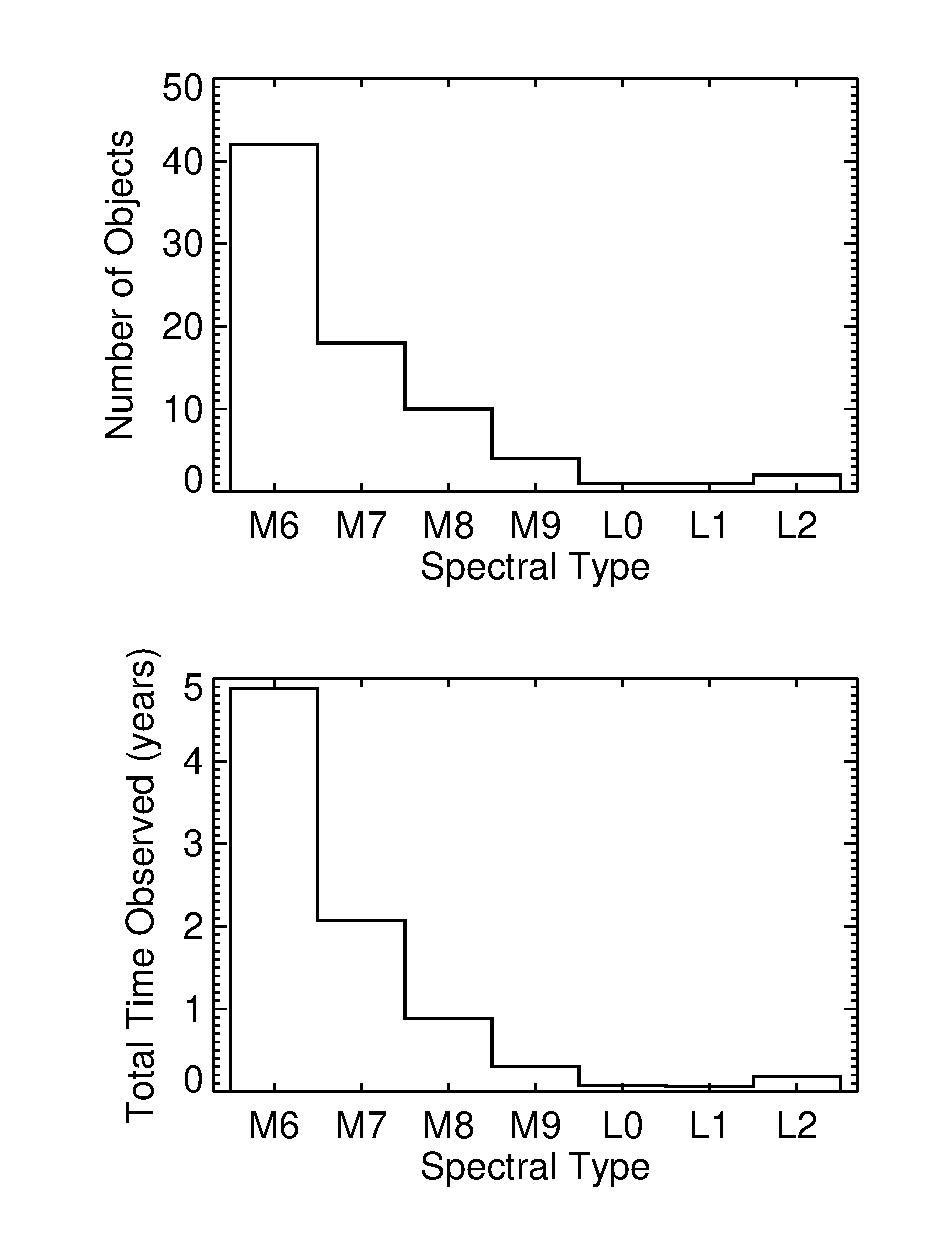
\includegraphics[width=0.5\columnwidth]{ST_stats.eps}
    \caption{Number of objects (top panel) and total time observed in TESS so far (bottom panel) as a function of spectral type for the TESS UCD cycle 1 short cadence sample. The strong decline, both in number of objects and time observed, is due both to early-type objects being more common and also to the declining brightness with later types.}
    \label{fig:ststat}
\end{figure}

To confirm that the lightcurves were accurately extracted from the target pixel files, we reviewed the aperture placement on the target pixel files (I haven't done them all yet, but I do want to -SJS). For targets where the extraction selected the appropriate source, we adopted the SAP flux from the lightcurve files. For the other targets, we re-extracted the lightcurves from the target pixel files using a magic incantation. 

\section{Rotation Analysis} \label{sec:rot}
\subsection{Variability amplitudes} \label{subsec:varamp}
\subsection{LC Morphologies} \label{subsec:LCmorph}

\section{Flares in the TESS UCD Sample} \label{sec:Flares}
We identified and found energies for our flares. 

\subsection{Flare Finding}
\label{subsec:findflare}
To find flares in the TESS UCD sample, we used the AltaiPony flare finding code \citep[][in prep.]{Ilin2019,Ilin2020}. Here, we should describe background fitting, picking out of flares, and measuring of amplitude, duration, and equivalent duration and their associated uncertainties. We also reviewed the flares by eye to confirm that each was a flare. We confirmed a total of \# flares on \# objects. 
%--------------------------------------------
\subsubsection{Custom apertures and de-trending}
TESS light curves have pre-defined aperture masks but for a number of targets they were shifted for reasons. We decided to re-extract all light curves manually, using the \texttt{lightkurve}~\citep{lightkurve2019} toolbox designed for Kepler/K2 and TESS data analysis. Consequently, we manually masked observing periods with strong systematics, that the internal TESS de-trending procedure would have otherwise accounted for, on a sector-by-sector basis.
\subsubsection{Light curve de-trending}
TESS UCD light curves exhibited various astrophysical and systematic trends. Removing them was necessary to enable searching the residual time series for flares with a simple, deterministic algorithm, and determining the quiescent flux nd noise properties of the light curve as accurately as possible. The main trends stemmed from the movement of the spacecraft, and stellar rotational modulation caused by spots.
\\
To account for these effects we arrived at the following procedure: If the difference in flux from the beginning to the end of the light curve was $>20,\%$ we fitted a cubic spline to the $12$ h binned light curve to remove strong global trends that take effect on time scales of multiple days. When no strong global trends were left, we removed strong rotational modulation iteratively using sine fits with periods obtained from  Lomb-Scargle periodograms~(\texttt{lightkurve.Periodogram}, see~\citealt{lomb1976,scargle1982}) until no strong periods were left in the light curve. To this end, we computed Signal-to-Noise Spectra from the periodograms using the \texttt{lightkurve.Periodogram.flatten()} method that divided out the noise background using a moving median where the filter width that grows logarithmically in frequency space.
Next, we removed remaining trends with using a rolling median on time scales of $10$ h, longer than the vast majority of flares was visible. To remove trends on shorter time scales, we masked outliers that could be flare candidates. We padded them with $25$ data points before and after each series of outliers. We applied a Savitzky-Golay~\citep{SavGol1964} filter (\texttt{scipy.signal.savgol\_filter},~\citealt{scipy2019}) with window sizes that were three times shorter that the dominant residual frequency in any continuous observing period. The Savitzky-Golay filter is known as a flexible high-pass filter in signal processing. We determined the dominant frequency using a Fast Fourier Transformation (FFT) from \texttt{scipy.fftpack}~\citep{scipy2019}. The minimum window size was $2.5$ h. In a final step we filtered the light curve with the minimum window size of 2.5 h, and estimated the scatter in the light curve using a rolling standard deviation (window size$= .5$ h) masking and padding positive outliers, i.e. flare candidates, as before. The masked regions in the light curve were assigned the mean uncertainty from the rest of the light curve. Thus we used the non-flaring parts of the light curve to determine the quiescent flux and noise propertiers.
\\
The timescale of rotational modulation for the fastest rotating stars came close or even fell below flare durations of a few observed events. Removing variability on these timescales with any kind of band pass filter would modify the flare signal, too.  resorting and removing sinusoidal signal with very short periods, however, circumvented this shortcoming. Stars that showed these multiperiod flares will be adressed elsewhere~(Ilin et al. (in prep.)).
\subsubsection{Amplitude, duration, ED and their uncertainties}
determine the noise properties: Use the flaring part of the LC to determine the flare properties, use the rest to estimate the noise properties. Even for the most active stars, flares do not take up more than \# \% observed time.
\\
ED is calculated as the area under the curve.
\\
uncertainty on the duration of the flares is dominated by the decay tail of the flare hiding in the noise and shortening the duration accordingly. On the other hand, the shortest flares cannot lift the minimum required three subsequent data points above the 3$\sigma$ threshold. Theoretically, extremely long, and low-amplitude flares, that barely exceed the noise limits may be levelled out by the de-trending procedure. But such flares have not been observed yet, not least because above a duration of a few hours low amplitude variability could also be spots or are longer-lived phenomena on the stellar surface. 
\subsubsection{Injection-recovery}

%---------------------------------------------
The distribution of flares with respect to spectral type is shown in Figure~\ref{fig:stflare}. The fraction of objects that flare and the overall flare rate both decline with spectral type. This is in direct contrast to the increase in number of objects showing magnetic activity in the H$\alpha$ emission line \citep{Schmidt2015}, but may instead trace the well-known decline in strength of that emission line. 

White light flares do exist on L dwarfs \citep{Schmidt2016a,Paudel2017}, and may simply be too rare at energies strong enough to be detected in our TESS short cadence sample. With the incomplete dataset, there's 5 sectors on L0 and later. I'd like to be able to say something a little more firm about whether the lack of flares is totally expected or not! 

\citep{Schmidt2015}
\begin{figure}
	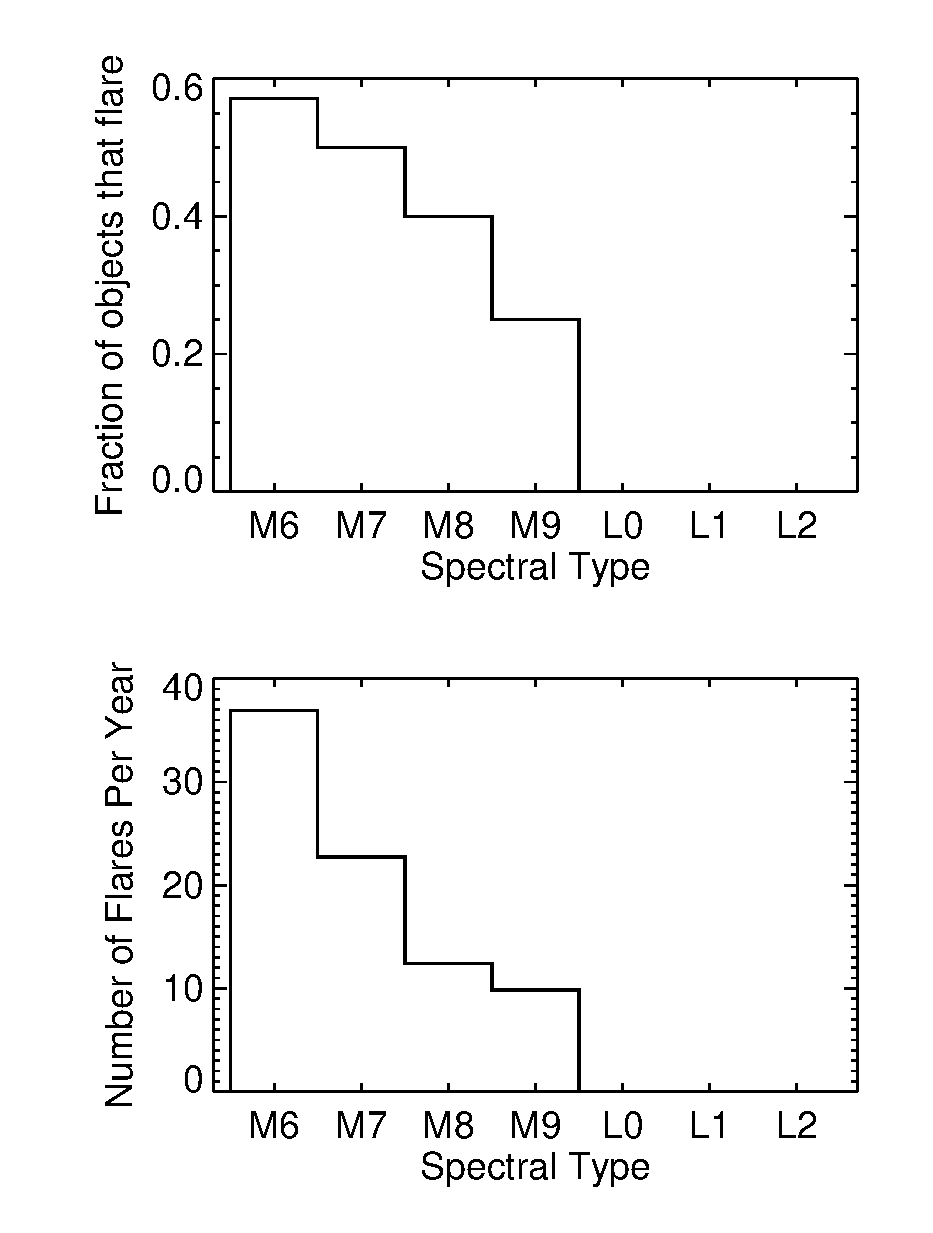
\includegraphics[width=0.5\columnwidth]{flare_stats.eps}
    \caption{Fraction of objects that flare (top panel) and number of flares per year (bottom panel) in the TESS UCD cycle 1 short cadence sample. The flaring fraction and the rate of flares both show a decline from M6 to L spectral types, with no flares yet found in L0 and later dwarfs.}
    \label{fig:stflare}
\end{figure}

Injection recovery, and how that affects our flares and the uncertainties. 

\subsection{Flare Energies from Quiescent UCD Luminosities} \label{subsec:tessmag}
To calculate energies for our flares, we multiplied the equivalent duration, measured from the TESS lightcurve, by the quiescent flux in the TESS band. To estimate the quiescent flux, we used spectrophotometry of template spectra of ultracool dwarfs \citep{Bochanski2007a,Schmidt2014a} combined with spectra from the SpeX library (cite or site or both I forget), anchored to their Gaia magnitudes \citep{Gaia-Collaboration2018}. 

We obtained updates TESS fluxes and magnitudes. Then calculated TESS luminosities using the distances from Gaia (nearby low uncertainty so 1/parallax is totally fine). 

And yes, I should figure out what to do for objects not in Gaia. 

\subsection{Flare Frequency distributions} \label{subsec:FFD}
The flare frequency distribution, binned by spectral type, is shown in Figure~\ref{fig:ffd}. Overall, the M6 and M7 dwarfs flare more than those in previous work. 

\begin{figure}
	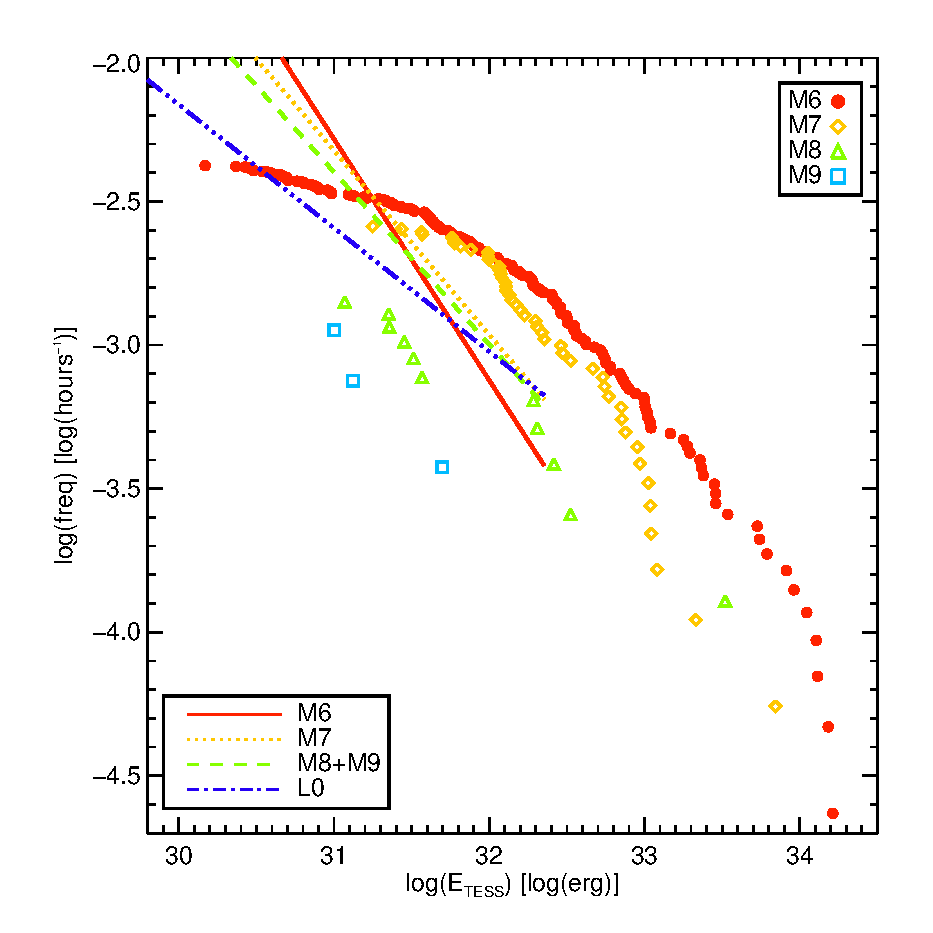
\includegraphics[width=0.5\columnwidth]{FFD_v6.eps}
    \caption{Log of flare frequency as a function of TESS band flare energy for the TESS Cycle 1 short cadence sample (individual symbols) and the K2 ultracool dwarfs of  \citet{Paudel2017}. The TESS observations overall extend to lower frequencies and higher energies due to the larger total observing time. The M6 and M7 dwarfs in TESS flare more strongly and frequently than those of K2, though the M8 and M9 dwarfs show only a handful of flares at lower energies and frequencies of K2.  }
    \label{fig:ffd}
\end{figure}

Here, we will probably also talk a lot about the power law fits. 

\subsection{Empirical flare template}\label{subsec:template}
GJ1243, a radiply rotating M4 dwarf with $P=0.592$\,d, was observed by the primary Kepler mission in 1 min cadence for 11 months. It was actively flaring with a total of 885 flares detected in the light curves~\citep{davenport2014}. From these a semi-empirical flare template was derived with a polynomial rise phase and two overlapping exponential decay phases, which has been widely used in later studies. We reproduced Figure 4 from~\citet{davenport2014} here with the flares in our sample, and fitted the template to the result. If the models are fully consistent, the best fit values for the template parameters will be $t_{peak}=1.$, $FWHM=1.$, and $a=1.$ within uncertainties.

\begin{figure}
	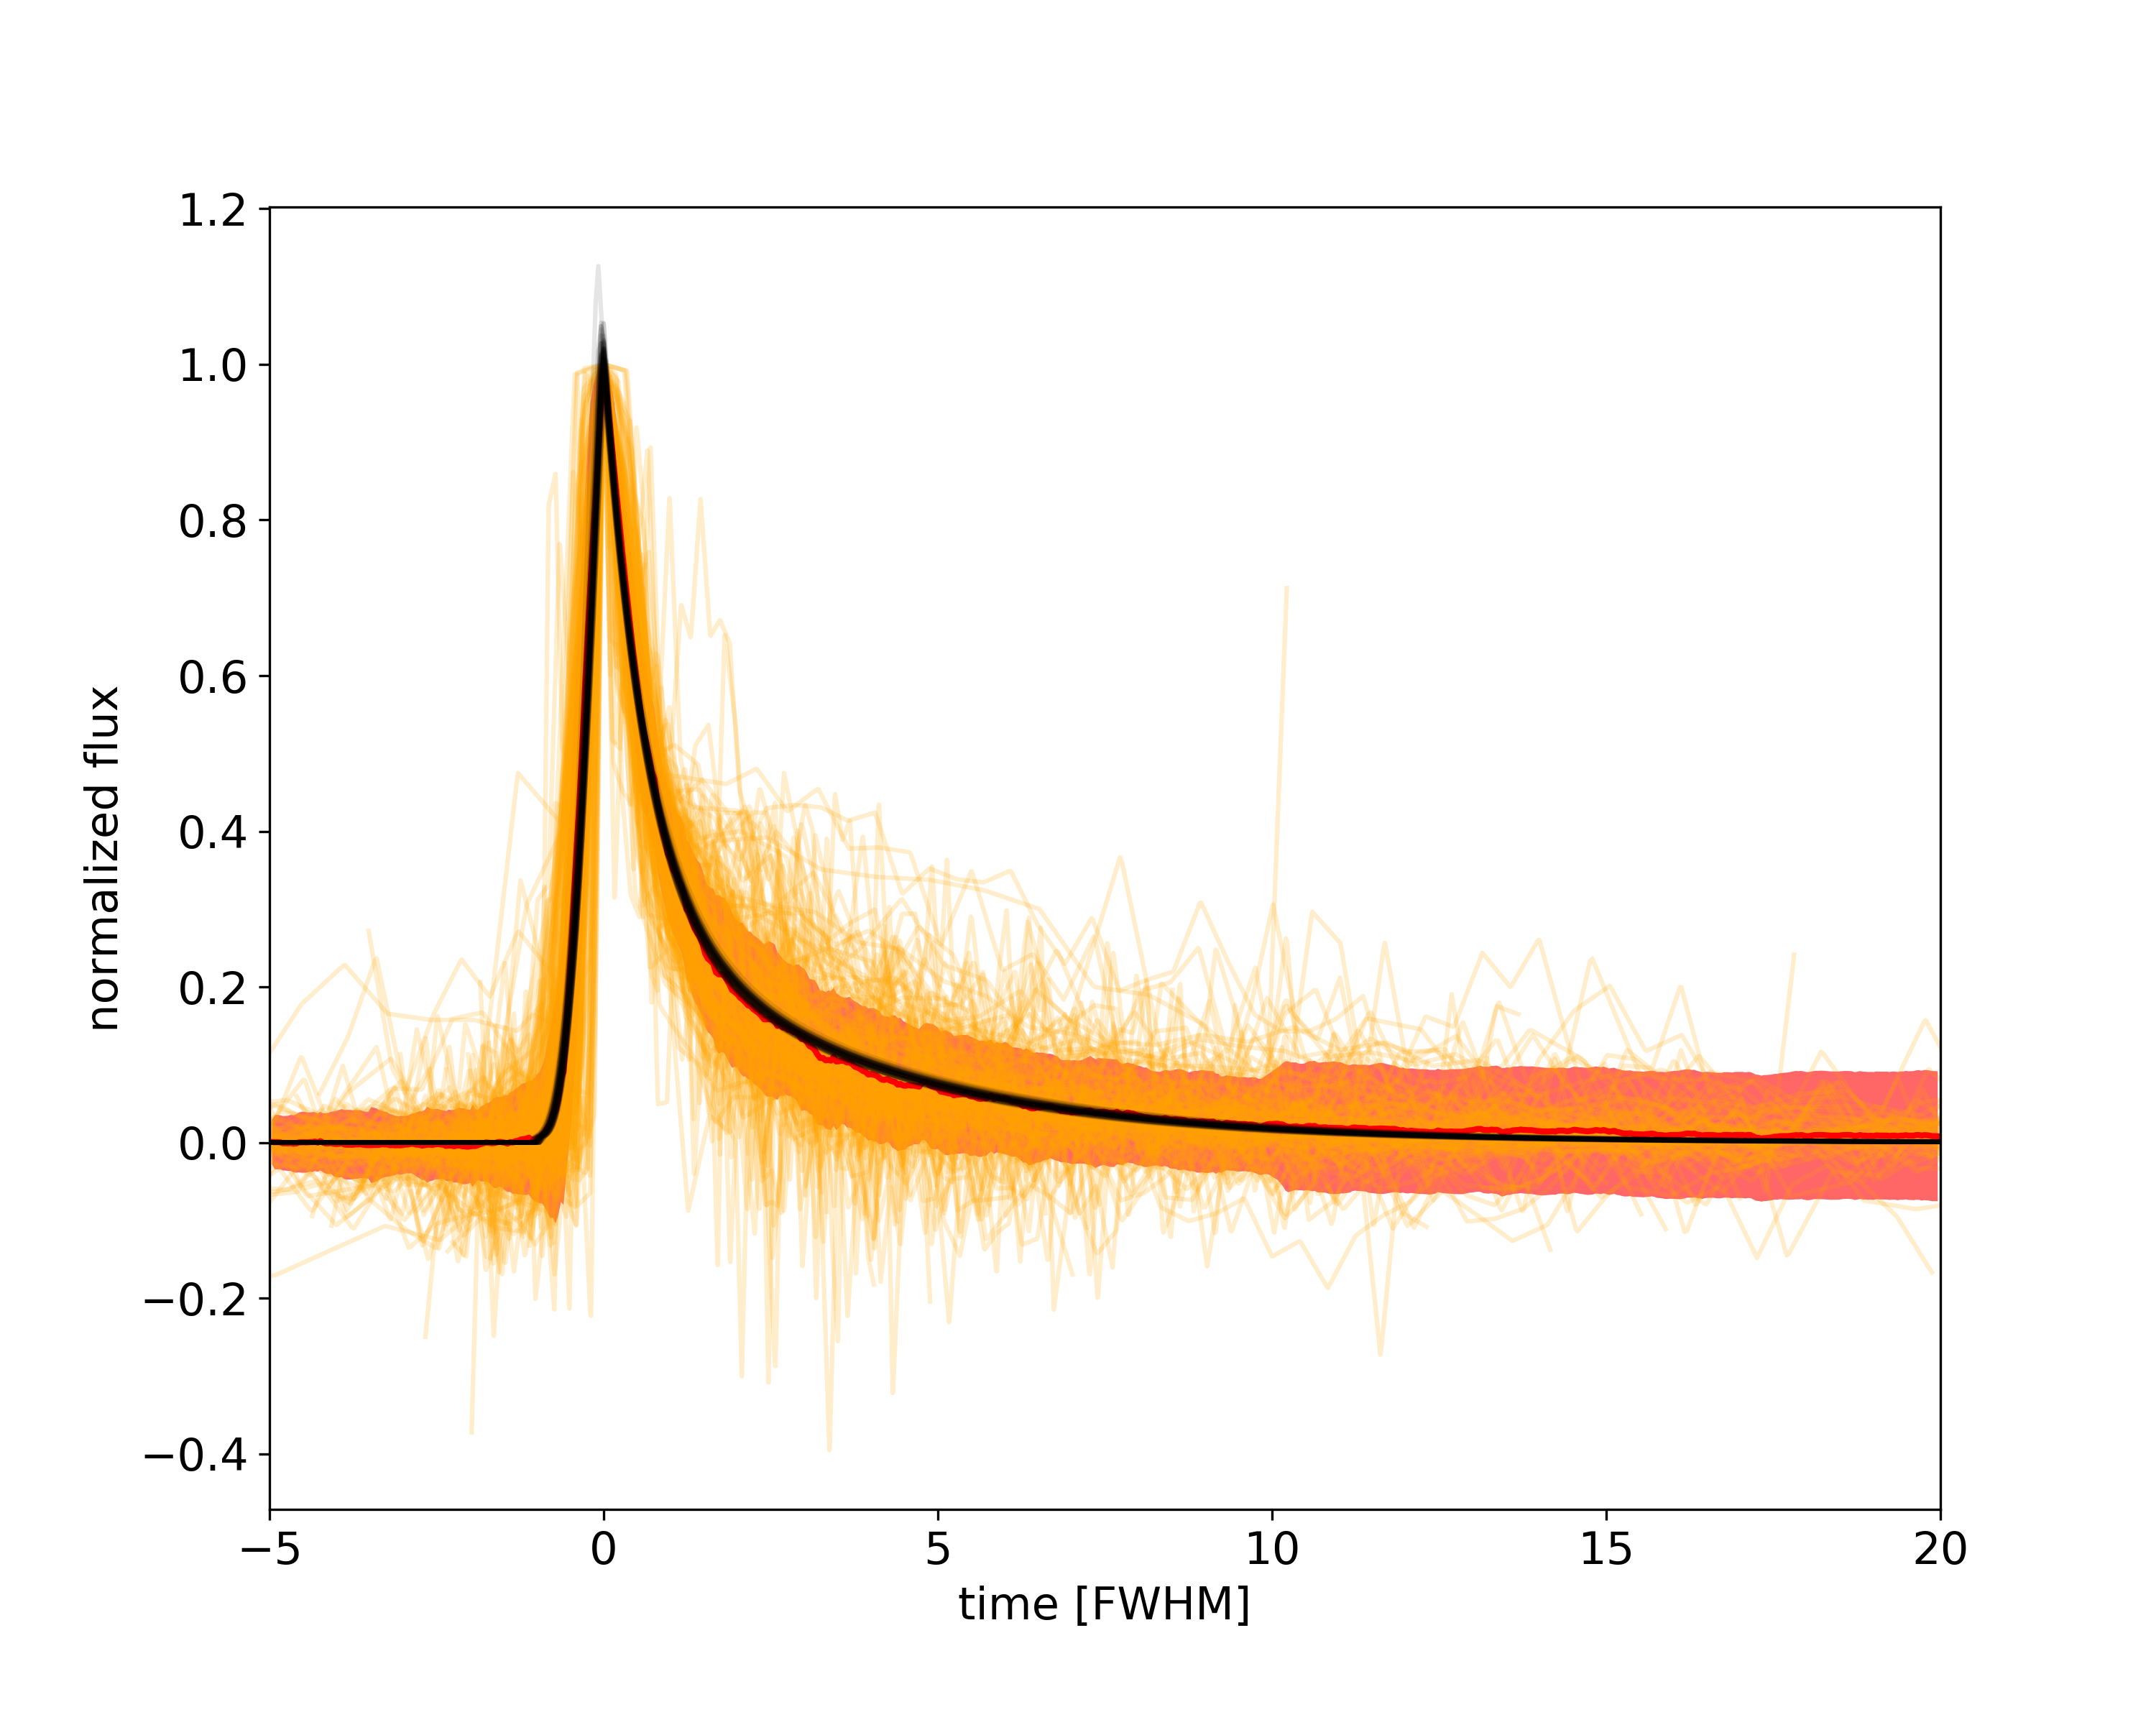
\includegraphics[width=0.5\columnwidth]{11_03_2020_11_15_all_davenport_fit_median_norel.png}
    \caption{Yellow: individual flare light curves. Black: Samples from the posterior distribution}
    \label{fig:template}
\end{figure}


\section{Summary/Conclusions} \label{sec:conclusion}


\acknowledgments

\vspace{5mm}
\facilities{}

\software{astropy~\citep{astropy2018}, astroquery~\citep{astroquery2019}.}

% it's a rather incomplete bib file, I'll add or feel free to add!
\bibliography{TESS_UCD} 


\end{document}


